\documentclass[11pt]{beamer}
\usepackage{color,soul}
\usepackage[utf8]{inputenc}
\usepackage{amsmath}
\usepackage{amsfonts}
\usepackage{amssymb}
\usepackage{algpseudocode} % uses algorithmicx package automatically
\usepackage{mathrsfs}
\usepackage{graphicx}
\DeclareMathOperator*{\argmin}{\mathbf{arg\,min}}
\DeclareMathOperator*{\argmax}{\mathbf{arg\,max}}
%\DeclareMathOperator*{\sup}{sup}
\DeclareMathOperator{\F}{\mathcal{F}} % Function Classes
\DeclareMathOperator{\FF}{\mathcal{F}} % prettier function classes
\DeclareMathOperator{\Hs}{\mathscr{H}} % Hilbert Spaces
\DeclareMathOperator{\R}{\mathbb{R}} % Reals
\DeclareMathOperator{\Rad}{\mathcal{R}} % Rademacher
\DeclareMathOperator{\E}{\mathbb{E}} % Expectation
\DeclareMathOperator{\Or}{\mathcal{O}} % Order Notation
\DeclareMathOperator{\Tr}{\textbf{Tr}} % Expectation
\DeclareMathOperator{\grad}{\nabla} % Gradient
\DeclareMathOperator{\LLH}{\mathcal{L}} % Log Likelihood etc.
\DeclareMathOperator{\Lag}{\mathcal{L}} % Lagrangian etc.
\DeclareMathOperator{\X}{\mathcal{X}} % input space X
\DeclareMathOperator{\Y}{\mathcal{Y}} % output space Y
\DeclareMathOperator{\bF}{\mathbf{F}} 
\DeclareMathOperator{\w}{\mathbf{w}} % weight vector
\DeclareMathOperator{\y}{\mathbf{y}} % output structure
\DeclareMathOperator{\x}{\mathbf{x}} % input structure
\DeclareMathOperator{\f}{\mathbf{f}} % function
\DeclareMathOperator{\K}{\mathcal{K}} % set of Kernels
\DeclareMathOperator{\vw}{\overrightarrow{w}} % set of Kernels
\DeclareMathOperator{\T}{\mathcal{T}} % set of Kernels

%\DeclareMathOperator{\implies}{\rightarrow} % implies

\newcommand{\opt}[1]{{#1}^{*}} % give f* for Optimal, Dual ...
\newcommand{\pred}[1]{\hat{#1}} % Prediction 
\newcommand{\dotprod}[2]{ \langle {#1} , {#2} \rangle } % <w,x> style
\renewcommand{\Pr}{\mathbb{P}} % Probability
\renewcommand{\vec}[1]{\mathbf{#1}} % vectors

\newcommand*{\Let}[2]{\State {#1} $\gets$ {#2}}

\usepackage{xcolor}

\newcommand{\highlight}[1]{\colorbox{yellow}{$\displaystyle #1$}}
\newcommand{\highlightmath}[1]{\colorbox{yellow}{\[\displaystyle #1\]}}


\author{Shyam Upadhyay}
\title{Qualifying Exam}

\setbeamercovered{transparent} 
\date{Shyam Upadhyay} 

\begin{document}

\begin{frame}
\titlepage
\end{frame}

\begin{frame}{About Me}
\begin{itemize}
\item Working with Dan Roth.
\item Interested in machine learning, dabble in NLP (I would like to be identified as a ML person instead of a linguist).
\item Publication in AAAI'15 on Learning with Amortized Inference.
\end{itemize}
\end{frame}

\begin{frame}{My Current Research}
Grounding Events to a Knowledge Base
\emph{After the death of Cromwell in 1658, Charles's chances of regaining the Crown at first seemed slim as Cromwell was succeeded as Lord Protector by his son, Richard.}

\end{frame}

\begin{frame}{Issues}
Only 1\% of wikipedia pages are about events.
Number higher if you consider events in subheading of a entities page eg. ``Invasion of Russia'' section under the wikipage of \textsc{Napolean}.
\end{frame}

\begin{frame}{Premise of the Paper}
  \begin{example}
    Test
  \end{example}
\end{frame}

%%%%%%%%%%%%%%%%%%%%%%%%%%%%%%%%%%%%%%%%%%%%%%%%%%
\begin{frame}
  \begin{center}
    {
      \huge GloVe: Global Vectors for Word Representation
    } \\
    Pennington,Socher,Manning
  \end{center}
\end{frame}

%%%%%%%%%%%%%%%%%%%%%%%%%%%%%%%%%%%%%%%%%%%%%%%%%%
\begin{frame}{Introduction}
  \begin{itemize}[<+->]
  \item How to represent a word in a machine?
    % coverage issues
  \item A mathematical representation of words as real valued vectors.
    %% way of representing a word as real valued (possibly dense) vector
    %% conventional way - one hot repr lead to data sparsity, does not take word relationships into account
  \item Representation captures some form of ``related-ness''.
    %% should express some notion of similarity b/w words
    \begin{figure}
      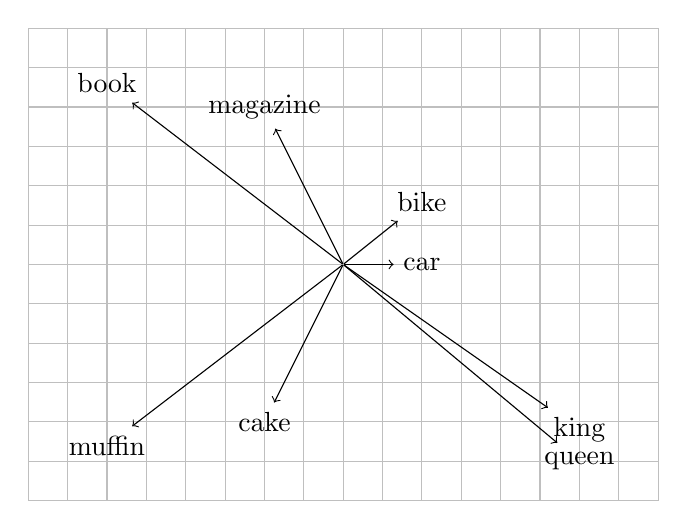
\begin{tikzpicture}
        \draw[step=0.5cm, gray!50] (-4,-3) grid (4,3); % good idea to have a grid
        \node (car) at (1,0) {car};
        \node (bike) at (1,0.8) {bike};
        \node (king) at (3,-2.1) {king};
        \node (queen) at (3,-2.5) {queen};
        \node (book) at (-3,2.3) {book};
        \node (magazine) at (-1,2) {magazine};
        \node (muffin) at (-3,-2.3) {muffin};
        \node (cake) at (-1,-2) {cake};
        \node[inner sep=0pt,minimum size=0.1pt] (origin) at (0,0) {};
        \onslide<3->{
          \path[draw,->] (origin)--(car);
          \path[draw,->] (origin)--(bike);
          \path[draw,->] (origin)--(king);
          \path[draw,->] (origin)--(queen);
          \path[draw,->] (origin)--(book);
          \path[draw,->] (origin)--(magazine);
          \path[draw,->] (origin)--(muffin);
          \path[draw,->] (origin)--(cake);
        }
      \end{tikzpicture}
      %% 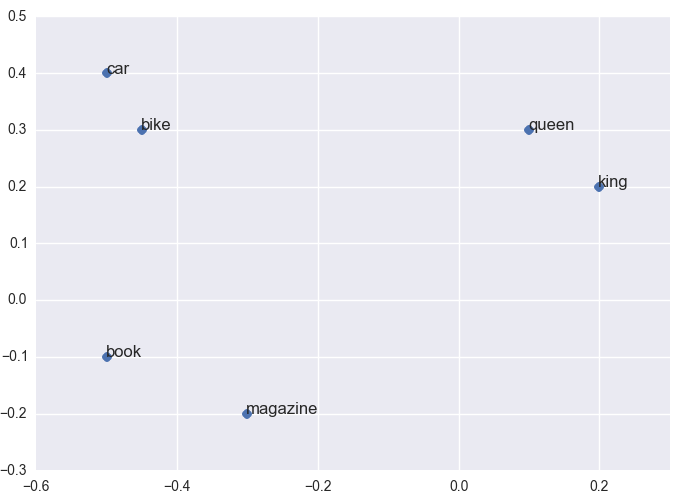
\includegraphics[scale=0.35]{images/wordvec.png}
      %% here is a 2d projection of vec for a few words. notice the cosine of the angles b/w them
    \end{figure}    
  \end{itemize}
\end{frame}



%% \begin{frame}
%%   \begin{center}
%%     {
%%       \huge Why Bother?
%%     } \\
%%   \end{center}
%%   \pause
%%   \begin{itemize}[<+->]
%%   \item Problem with Conventional Methods
%%     \begin{itemize}[<+->]
%%     \item meaning is lost.
%%     \item loses generalizability
%%     \item too much luggage.
%%     \end{itemize}
%%   \item Distributional Hypothesis to the rescue!
%%   \end{itemize}
%% \end{frame}

%%%%%%%%%%%%%%%%%%%%%%%%%%%%%%%%%%%%%%%%%%%%%%%%%%
\begin{frame}{Obtaining Vector Representations}
  Word vectors can be obtained in the following ways:
  \begin{itemize}[<+->]
  \item Cooccurence Matrix Factorization ~\cite{Deerwester}
    % LSA,PCA,HAL the name of the game is compute co-occurence
    % cmopute co-occurence and use a standard dim red technique
  \item Learn representation from Local Context ~\cite{Mikolov13a}.
    %% \item Sometimes just using the explicit context representation suffices ~\cite{Levy14}.
    %% Sometimes these methods end-up modeling the same objective (skip-gram).
    %% what abt random sampling?
  \end{itemize}
  %% Say its task specific, therefore there has been a explosion of papers on this topic.
  %% This paper proposes another way of obtaining word vectors via matrix factorization.
  %% They claim that their model combines advantages of both global and local? (??)
\end{frame}

%%%%%%%%%%%%%%%%%%%%%%%%%%%%%%%%%%%%%%%%%%%%%%%%%%
\begin{frame}{Motivation of the Paper}
  The configuration of the vectors encode relationships between words.
  %% Word vectors capture linguistic regularities in a simple manner.
  \begin{align*}
    vec(king) - vec(man) + vec(woman) \approx vec(queen)
  \end{align*}
  \visible<1->{
    \begin{figure}
      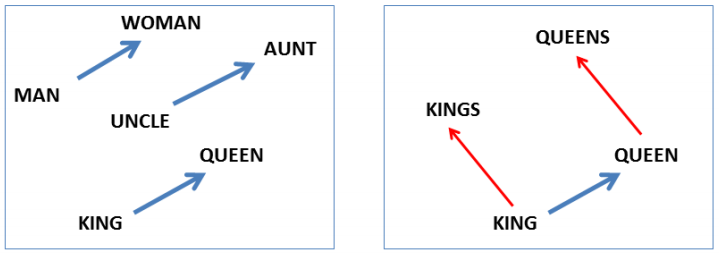
\includegraphics[scale=0.35]{images/mikolov.png}
      \caption{From ~\cite{Mikolov13a}}
      %% vectors offsets illustrate the gender relation. another projection illustrate plurality.
    \end{figure}
  }
  \onslide<2->
  This paper claims that they explicitly model the properties needed for achieving the above effect.
  %% No explanation was given in the original papers.
  %% Remarkably, training such a lexical model induces word repr. with striking semantic and syntactic properties---\cite{Mikolov13a}
  %% Levy showed that tranditional methods like count sparse contexts can perform equally well.
  %% ... traditional word similarities can perform just as well as neural embeddings ---\cite{Levy14}
  %% talk about Dont Count Predict paper
\end{frame}

\begin{frame}{Why is this Useful?}
  \onslide<1->{
    \begin{exampleblock}{Questions Like..}
    \begin{center}
      man:king :: woman: ?
    \end{center}
    \end{exampleblock}
  }
  \onslide<2->{
    %% \begin{center}
    %%   So easy to answer now!
    %% \end{center}
    \begin{align*} 
    \only<2> {\min_x \qquad \|x - (king - man + woman)\|^2 \\}
    \only<3-> {\max_x \qquad \dotprod{x}{king} - \dotprod{x}{man} + \dotprod{x}{woman} \\}
    \end{align*}
  }
\end{frame}
%% Global Matrix Factorization Methods are prone to ill-effects of predominance of function words.
%%%%%%%%%%%%%%%%%%%%%%%%%%%%%%%%%%%%%%%%%%%%%%%%%%
\begin{frame}{GloVe Model - What We Want}
  \begin{exampleblock}{Question}
    steam: gas :: ice:?
    \pause
    \begin{itemize}[<+->]
    \item Solid
    \item Gas
    \item Water
    \item Fashion
    \end{itemize}
  \end{exampleblock}
  \onslide<6->
  Ideally,
  \begin{align*} 
  steam - gas + solid &= ice \\
  steam - ice &= gas - solid \\
  \end{align*}
\end{frame}

%%%%%%%%%%%%%%%%%%%%%%%%%%%%%%%%%%%%%%%%%%%%%%%%%%
\begin{frame}{GloVe Model - Insight}
  \begin{exampleblock}{Desired}
    \begin{align*} 
      steam - ice &= gas - solid
    \end{align*}    
  \end{exampleblock}
  \begin{figure}[scale=0.8]
    %% 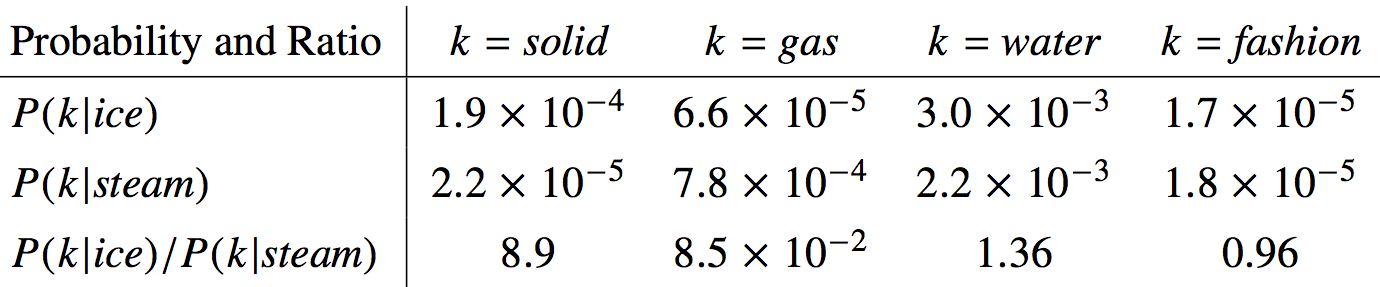
\includegraphics[scale=0.23]{images/glove_int.png}
    \begin{tabular}{c|cccc}
       & $k=solid$ & $k=gas$ & $k=water$ & $k=fashion$\\
      \hline
      $\Pr(k \mid ice)$ & \only<1-2>{$1.9 \times 10^{-4}$}\only<3->{large} & \only<1-2>{$6.6 \times 10^{-5}$}\only<3->{small} & \only<1-2>{$3.0 \times 10^{-3}$}\only<3->{large} & \only<1-2>{$1.7 \times 10^{-5}$}\only<3->{small} \\
      $\Pr(k \mid steam)$ & \only<1-2>{$2.2 \times 10^{-5}$}\only<3->{small} & \only<1-2>{$7.8 \times 10^{-4}$}\only<3->{large} & \only<1-2>{$2.2 \times 10^{-3}$}\only<3->{large} & \only<1-2>{$1.8 \times 10^{-5}$}\only<3->{small} \\
      \visible<2->{
       $\frac{\Pr(k \mid ice)}{\Pr(k \mid steam)}$ & \only<2>{$8.9$}\only<3->{large} & \only<2>{$8.5 \times 10^{-5}$}\only<3->{small} & \only<2>{$1.36$}\only<3->{$\sim 1$} & \only<2>{$0.96$}\only<3->{$\sim 1$}
      }
    \end{tabular}
  \end{figure}
  %% the ratio helps discriminate the words that distinguish ice from stream.
  %% in cases like water and fashion the affinity/dissimilarity is almost the same, 
  %% whereas in solid and gas the affinity shifts towards a particular related word
  \visible<4->{
    \begin{center}
      Ratio indicates affinity to choose b/w two words.
    \end{center}
  }
\begin{center} 
  \only<5>{Word likes neither $\implies \frac{\Pr(k \mid ice)}{\Pr(k \mid steam)} \sim 1$}
  \only<6>{Word prefers ice over steam $\implies \frac{\Pr(k \mid ice)}{\Pr(k \mid steam)} \gg 1$}
  \only<7>{Word prefers steam over ice $\implies \frac{\Pr(k \mid ice)}{\Pr(k \mid steam)} \ll 1$}
\end{center}  
\end{frame}

\begin{frame}{The Intuition behind the Model}
  
  \begin{exampleblock}{Intuition}
    %% If a word prefers ice over steam, it will also prefer solid over gas. If it prefers neither, then it will prefer neither between solid and gas.
  \begin{align*}
    \frac{\Pr(k \mid ice)}{\Pr(k \mid steam)} \approx \frac{\Pr(k \mid solid)}{\Pr(k \mid gas)} \Forall k
  \end{align*}
  \end{exampleblock}
  \begin{center} 
    \only<2>{So lets work with conditional probabilities and take ratios!}
    \only<3->{\st{So lets work with conditional probabilities and take ratios!\\}}
    \onslide<3->{
      Too cumbersome! \\
      %% Need a compact representation.
    }
  \end{center}
\end{frame}

\begin{frame}{Approximate with Vectors Representations}
  Demand that,
  \begin{align*} 
      \onslide<1->{
        w_i^Tw_j &= \log \Pr(j\mid i) \\
      }
      \onslide<2->{
        \underbrace{(w_{ice}-w_{steam})^T}_{\text{``probe to check affinity''}} w_j &= \log\frac{\Pr(j \mid ice)}{\Pr(j \mid steam)} \\
      }
      \onslide<3->{
        (w_{solid}-w_{gas})^T w_j &= \log\frac{\Pr(j \mid solid)}{\Pr(j \mid gas)} \\
      }
      \onslide<4->{
        (w_{ice}-w_{steam})^T w_j & \approx (w_{solid}-w_{gas})^T w_j \\
      }
      \onslide<5->{
        w_{ice}-w_{steam} & \approx w_{solid}-w_{gas}
      }
    \end{align*}
    \onslide<6->
    \begin{center} 
      \Huge{
        Is this new?
      }
    \end{center}
\end{frame}
%%%%%%%%%%%%%%%%%%%%%%%%%%%%%%%%%%%%%%%%%%%%%%%%%%
\begin{frame}{GloVe Model - Derivation of Objective}
  Let co-occurence matrix be $X$.
  \begin{align*}
    %% & \Pr(\text{word j appears in context of word i}) = \Pr_{ij} \\
    %% \visible<1->{& \Pr_{ij} \propto \exp({w_i}^T{\tilde{w}_j}) \tag{log-bilinear model} \\}
    \visible<2->{& w_i^T\tilde{w_j} = \log X_{ij} - \log X_{i} \tag{$\Pr(k \mid i)=\frac{X_{ik}}{X_i}$} \\}
    %% & \frac{\Pr_{ik}}{\Pr_{jk}}=\exp(\dotprod{w_i -w_j}{\tilde{w}_k}) \\
    %% & \log \Pr_{ik} - \log\Pr_{jk} = \dotprod{w_i -w_j}{\tilde{w}_k}\\
    \visible<3->{& w_i^T\tilde{w_j} +b_i = \log X_{ij}} \\
    \visible<4->{& w_i^T\tilde{w_j} +b_i + \tilde{b_j} = \log X_{ij}}
  \end{align*}
  \visible<5->{
    We can minimize 
    \begin{align*}
      & \sum_{i=1,j=1}^V \left( w_i^T\tilde{w_j} +b_i + \tilde{b_j} - \log X_{ij} \right)^2
    \end{align*}
  }
  %% note the similarity with matrix factorization
  \begin{center}
    \visible<6->{But wait!}
  \end{center}
  %% The problem is that X_ij are estimated from data. Some values will be very large/small (most of them will be zero), so our learning algo will waste effort on optimizing to fit the useless entries.
\end{frame}

%%%%%%%%%%%%%%%%%%%%%%%%%%%%%%%%%%%%%%%%%%%%%%%%%%
\begin{frame}{GloVe Model - Introduce Weighted Cost}
  \begin{align*}
    & J = \sum_{i=1,j=1}^V \alert{f(X_{ij})} \left( w_i^T\tilde{w_j} +b_i + \tilde{b_j} - \log X_{ij} \right)^2
  \end{align*}
  
  \visible<2->{
    %% \begin{center}
    %%   $f$ should not overweight rare and too-frequent co-occurences.
    %% \end{center}
    %% f should clip values above a certain threshold
    \begin{align*}
      f(x)=
      \begin{cases}
        (x/x_{max})^\alpha & \text{ if $x < x_{max}$} \\
        1 & \text{ otherwise}
      \end{cases}
      %% explain what x_max and \alpha do
      %% x_max prevents too-freq to overweigh
      %% large alpha means underweigh rare occurences more severely
    \end{align*}
  }
  \visible<3->{
    \begin{figure}
      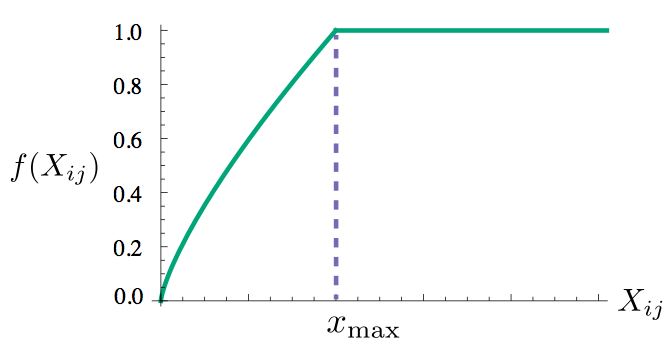
\includegraphics[scale=0.27]{images/weighting.png}
      \caption{$f$ with $\alpha=3/4$}
    \end{figure}
  }
\end{frame}

%%%%%%%%%%%%%%%%%%%%%%%%%%%%%%%%%%%%%%%%%%%%%%%%%%
%% \begin{frame}{Model Parameters and Training}
%%   \begin{itemize}
%%   \item $x_{max},\alpha$
%%   \item window size, vector dimension
%%   \item corpus size
%%   \end{itemize}
%%   \begin{itemize}[<+->]
%%   \item Compute $X$
%%   \item $J$ is optimized using SGD.
%%   \end{itemize}
%% \end{frame}

%%%%%%%%%%%%%%%%%%%%%%%%%%%%%%%%%%%%%%%%%%%%%%%%%%
%% \begin{frame}{Model Analysis}
%%   \begin{itemize}
%%   \item Vector Length:
%%   \item Context Size: 
%%   \item Corpus Size: nothing suprising
%%   \item Model trained on smaller wikipedia corpus( 1.6B tokens) does better on semantic task than model trained on larger corpus like gigaword (4.3B tokens)
%%   \item Idea: instead of using only word vector $w$, use $w+c$, where $c$ is the context vector (significant improvement in semantic task). This can be used for other models as well.
%%   \end{itemize}
%% \end{frame}

%%%%%%%%%%%%%%%%%%%%%%%%%%%%%%%%%%%%%%%%%%%%%%%%%%
\begin{frame}{Training and Evaluation}
  \begin{exampleblock}{Training}
    \begin{itemize}[<+->]
    \item Compute co-occurence matrix $X$.
      %% this is a batch computation
    \item Do SGD alternatingly.
      %% you sample a entry from X, compute grad and descend
    \end{itemize}
    \onslide<3->{\textsc{Parameters:} vector dim., context size, corpus, $x_{max},\alpha$, iterations}
    %% wide range of parameters that you can play with, and they do have effect
  \end{exampleblock}
  \onslide<4->
  \begin{alertblock}{Evaluation}
    %% we will evaluate the model on 3 fronts
    \begin{itemize}[<+->]
    \item Semantic Relatedness % (Google Dataset) % intrinsic
      %% assess how good the vectors are at finding semantic relatedness
      \begin{itemize}
      \item \textsc{Putin} is to \textsc{Russia} as \textsc{Sarkozy} is to ? (\textsc{France})
      \end{itemize}
    \item Syntactic Relatedness % (Google dataset, MSR dataset) % intrinsic
      \begin{itemize}
      \item \textsc{Car} is to \textsc{Cars} as \textsc{Family} is to ? (\textsc{families})
      \end{itemize}
    \item Word Similarity
      \begin{itemize}
      \item Is \textsc{Tiger} more similar to \textsc{Cheetah} or \textsc{Mouse}?
        \end{itemize}
    %% \item NER 
    %%   \begin{itemize}
    %%   \item Uses word vectors as continuous features in a NER system.
    %%   \end{itemize}
    \end{itemize}
  \end{alertblock}
\end{frame}

%%%%%%%%%%%%%%%%%%%%%%%%%%%%%%%%%%%%%%%%%%%%%%%%%%
\begin{frame}{Results on Analogy Discovery}
  %% \begin{figure}
  %%   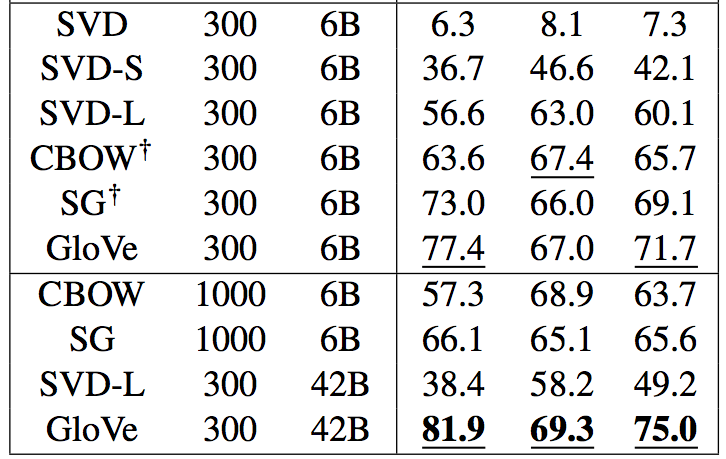
\includegraphics[scale=0.27]{images/results1_1.png}
  %% \end{figure}
  \begin{figure}
    \centering
    \begin{tabular}{|ccc|ccc|}
      \hline
      Model & Dim. & Size & Sem. & Syn. & Tot.\\
      \hline
      \textbf<2>{\color<2>{red}{SG}} & 300 & 1B & 61.0 & 61.0 & 61.0\\
      \textbf<2>{\color<2>{red}{CBOW}} & 300 & 1.6B & 16.1 & 52.6 & 36.1\\
      GloVe & 300 & \textbf<4-5>{\color<4-5>{blue}{1.6B}} & \textbf<4>{\color<4>{blue}{\underline{80.8}}} & \textbf<5>{\color<5>{blue}{\underline{61.5}}} & \underline{70.3}\\
      \hline
      SVD & 300 & 6B & 6.3 & 8.1 & 7.3\\
      %% SVD-S & 300 & 6B & 36.7 & 46.6 & 42.1\\
      \textbf<3>{\color<3>{blue}{SVD-L}} & 300 & 6B & \textbf<3>{\color<3>{blue}{56.6}} & \textbf<3>{\color<3>{blue}{63.0}} & \textbf<3>{\color<3>{blue}{60.1}}\\
      CBOW & 300 & 6B & 63.6 & \underline{67.4} & 65.7\\
      SG & 300 & 6B & 73.0 & 66.0 & 69.1\\
      GloVe & 300 & \textbf<4-5>{\color<4-5>{blue}{6B}} & \textbf<4>{\color<4>{blue}{\underline{77.4}}} & \textbf<5>{\color<5>{blue}{\underline{67.0}}} & \underline{71.7}\\
      \hline
      \textbf<2>{\color<2>{red}{CBOW}} & 1000 & 6B & 57.3 & 68.9 & 63.7\\
      \textbf<2>{\color<2>{red}{SG}} & 1000 & 6B & 66.1 & 65.1 & 65.6\\
      \textbf<3>{\color<3>{blue}{SVD-L}} & 300 & 42B & \textbf<3>{\color<3>{blue}{38.4}} & \textbf<3>{\color<3>{blue}{58.2}} & \textbf<3>{\color<3>{blue}{49.2}}\\
      GloVe & 300 & 42B & \underline{81.9} & \underline{69.3} & \underline{75.0}\\
      \hline
    \end{tabular}
    \caption{\% accuracy on analogy discovery}
    %% let me explain the models being compared
    %% first these numbers are not a fair comp.
    %% SVD-L degrades with more data.
    %% For semantic rel. more data does not mean better perf.
  \end{figure}
\end{frame}

%%%%%%%%%%%%%%%%%%%%%%%%%%%%%%%%%%%%%%%%%%%%%%%%%%
\begin{frame}{Results on Word Similarity}
  \begin{figure}
    %% 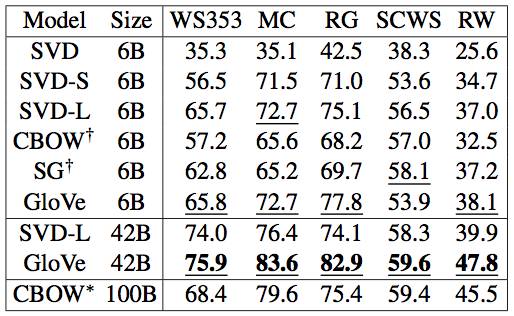
\includegraphics[scale=0.4]{images/results2.png}
    %% $\rotatebox[origin=c]{90}{time}
    %% \left\Downarrow
    \begin{tabular}{|cc|ccccc|}
      \hline
      Model & Size & WS353 & MC & RG & SCWS & RW\\
      \hline
      %% {SVD} & 6B & 35.3 & 35.1 & 42.5 & 38.3 & 25.6 \\
      %% \alert<2->{SVD-S} & 6B & 56.5 & 71.5 & 71.0 & 53.6 & 34.7\\
      \textbf<2>{\color<2>{blue}{SVD-L}} & 6B & \textbf<2>{\color<2>{blue}{65.7}} & \textbf<2>{\color<2>{blue}{63.0}} & \textbf<2>{\color<2>{blue}{60.1}} & \textbf<2>{\color<2>{blue}{56.5}} & \textbf<2>{\color<2>{blue}{37.0}}\\
      CBOW & 6B & 57.2 & 65.6 & 68.2 & 57.0 & 32.5\\
      SG & 6B & 62.8 & 65.2 & 69.1 & 58.1 & 37.2\\
      GloVe & 6B & {\bf 65.8} & {\bf 72.7} & {\bf 77.8} & {\bf 53.9} & {\bf 38.1}\\
      \hline
      \textbf<2>{\color<2>{blue}{SVD-L}} & 42B & \textbf<2>{\color<2>{blue}{74.0}} & \textbf<2>{\color<2>{blue}{76.4}} & \textbf<2>{\color<2>{blue}{74.1}} & \textbf<2>{\color<2>{blue}{58.3}} & \textbf<2>{\color<2>{blue}{39.9}}\\
      GloVe & 42B & {\bf 75.9} & {\bf 83.6} & {\bf 82.9} & {\bf 59.6} & {\bf 47.8}\\
      \hline
      %% \color<4->{red}{CBOW} & 100B & 68.4 & 79.6 & 75.4 & 59.4 & 45.5\\
      %% \hline
    \end{tabular}
    %% \right\downarrow
    %% \rotatebox[origin=c]{90}{time}$
    \caption{Spearman's correlation on word similarity with 300 dim. vectors.}
  \end{figure}
\end{frame}

%%%%%%%%%%%%%%%%%%%%%%%%%%%%%%%%%%%%%%%%%%%%%%%%%%
%% \begin{frame}{Results on NER}
%%   \begin{figure}
%%     %% 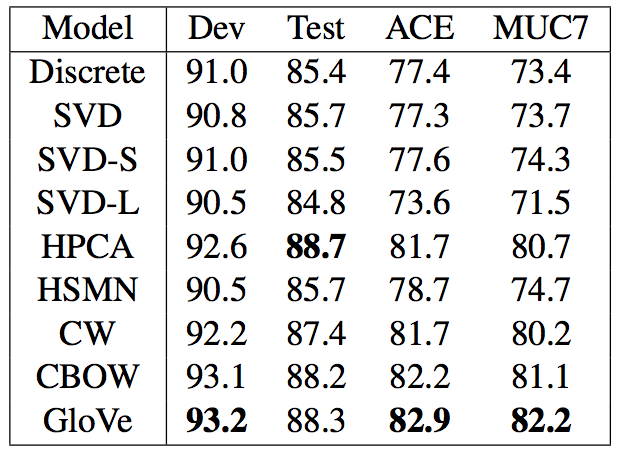
\includegraphics[scale=0.4]{images/ner.png}
%%     \begin{tabular}{|c|cccc|}
%%       \hline
%%       Model & Dev & Test & ACE & MUC7 \\
%%       \hline
%%       Discrete & 91.0 & 85.4 & 77.4 & 73.4\\
%%       SVD & 90.8 & 85.7 & 77.3 & 73.7\\
%%       SVD-S & 91.0 & 85.5 & 77.6 & 74.3\\
%%       SVD-L & 90.5 & 84.8 & 73.6 & 71.5\\
%%       %% HPCA & 92.6 & 88.7 & 81.7 & 80.7 \\
%%       %% CW & 92.2 & 87.4 & 81.7 & 80.2\\
%%       CBOW & 93.1 & 88.2 & 82.2 & 81.1\\
%%       GloVe & 93.2 & 88.3 & 82.9 & 82.2\\
%%       \hline
%%     \end{tabular}
%%     \caption{F1 on NER with 50d vectors.}
%%     %% say CBOW and Glove are comparable
%%     %% say why ACE vs MUC.
%%     %% Better ways of doing this?
%%   \end{figure}
%% \end{frame}


%%%%%%%%%%%%%%%%%%%%%%%%%%%%%%%%%%%%%%%%%%%%%%%%%%
%% \begin{frame}{Choice of Corpus}
%%   \begin{figure}
%%     \centering
%%     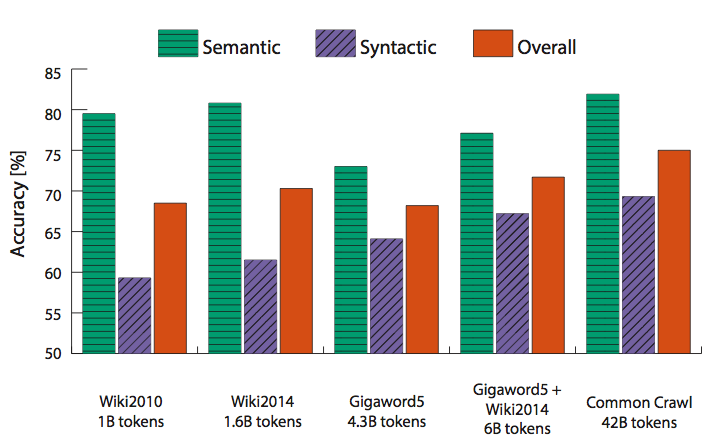
\includegraphics[scale=0.4]{images/corpus.png}
%%     %% \begin{subfigure}[b]{0.33\textwidth}
%%     %%   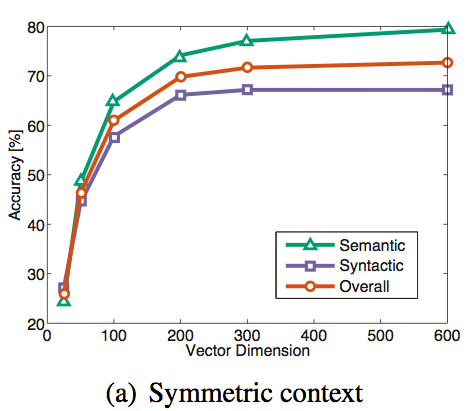
\includegraphics[width=\textwidth]{images/analogy1.png}
%%     %% \end{subfigure}%
%%     %% \begin{subfigure}[b]{0.33\textwidth}
%%     %%   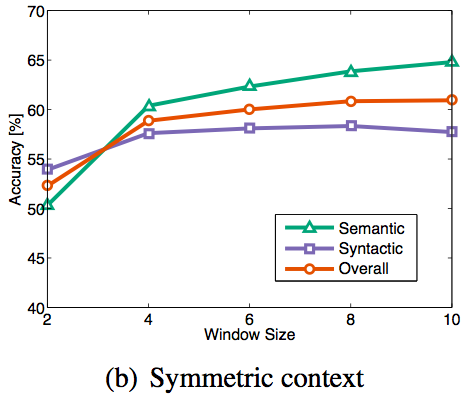
\includegraphics[width=\textwidth]{images/analogy2.png}
%%     %% \end{subfigure}%
%%     %% \begin{subfigure}[b]{0.33\textwidth}
%%     %%   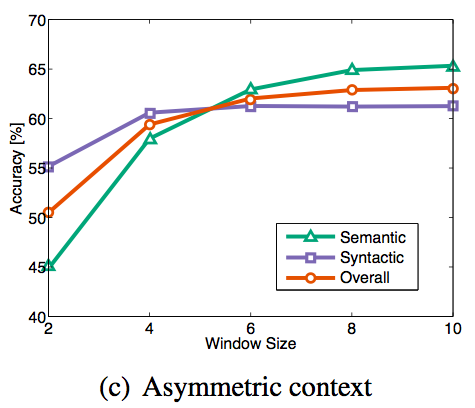
\includegraphics[width=\textwidth]{images/analogy3.png}
%%     %% \end{subfigure}%
%%   \end{figure}
%% \end{frame}

%%%%%%%%%%%%%%%%%%%%%%%%%%%%%%%%%%%%%%%%%%%%%%%%%%

%% \begin{frame}{GloVe vs. word2vec}
%%   \begin{figure}
%%     \centering
%%     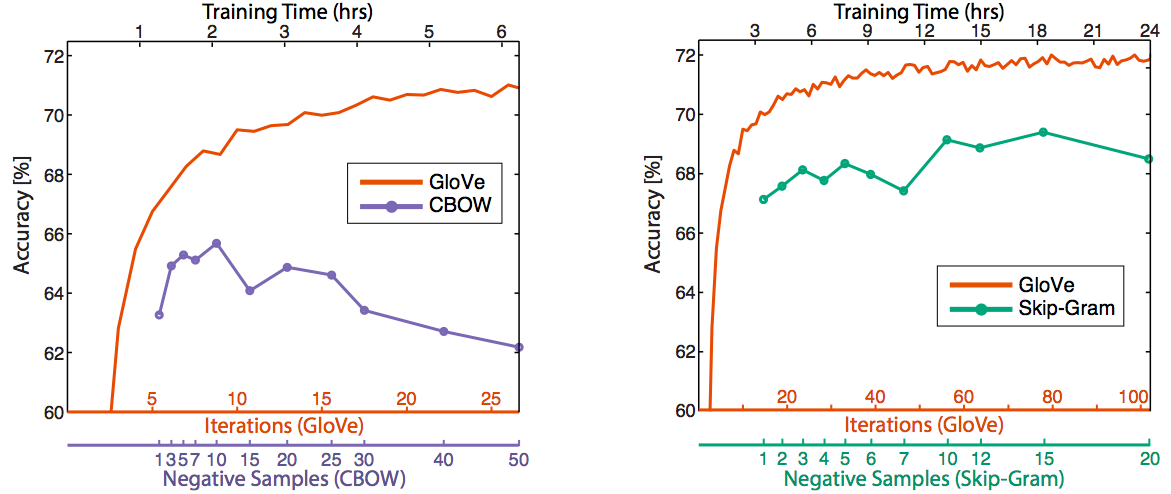
\includegraphics[scale=0.29]{images/gloveVSword2vec.png}
%%     \caption{Runtime and Accuracy Comparison}
%%     %% take this with a pinch of salt
%%   \end{figure}
%% \end{frame}

%%%%%%%%%%%%%%%%%%%%%%%%%%%%%%%%%%%%%%%%%%%%%%%%%%
\begin{frame}{Conclusion}
  \begin{itemize}[<+->]
    %% Boils down the task of learning representations to a bare minimum
    %% \item Matrix Factorization and Learning from Local Context are not that different.
  \item Nice formulation
  \item Age-old methods also work very well!
    %% \item Few experiments were not entirely fair, but ...
  \item Need of a standardized evaluation?
  \item Batch Computation?
  \item Interpretable vectors?
  \end{itemize}
\end{frame}

  %% new ideas from Turian Ratinov Bengio,
  %% curriculum training strategy?
  %% liang's preprocessing
  %% connotation vs denotation
  %% distributional vs distributed
  %% exp not done MSR dataset,
  %% batch restriction for glove vs online training for skip gram


\begin{frame}
  \begin{center}
    {\huge A* Sampling
    } \\
    Maddison,Tarlow,Minka
  \end{center}
\end{frame}

%% \begin{frame}{Premise of the Paper}
%%   %% what is the paper trying to solve
%% \end{frame}


%%%%%%%%%%%%%%%%%%%%%%%%%%%%%%%%%%%%%%%%%%%%%%%%%%
\begin{frame}{Partition Function Woes}
  Gibbs Distribution
  \begin{align*}
    \Pr(\x;\theta) =\frac{\exp(\theta^T\phi(\x))}{Z} \tag{$Z=\sum_{\x} \theta^T\phi(\x)$ is partition function}
  \end{align*}
  ML parameter estimation,
  \begin{align*}
    - \nabla_\theta \log LLH = \E_{\Pr(x;\theta)}\left[\phi(\x)\right] - \frac{1}{T} \sum_i\phi(x_i)
  \end{align*}
  Computing $\E_{\Pr(x;\theta)}$ is not usually tractable (Sampling from posterior is hard).
  Resort to approximations - MCMC, Contrastive Divergence etc.
\end{frame}

%%%%%%%%%%%%%%%%%%%%%%%%%%%%%%%%%%%%%%%%%%%%%%%%%%
\begin{frame}{Gumbel Distribution}
  \begin{align*}
    & Gumbel(m) = \text{gumbel with location parameter $m$}\\
    %% & CDF(x;\mu) = \exp \left(-\exp\left(-x+\mu\right)\right) \\
    & F_m(g) = \Pr(G\le g) = \exp(-\exp(-g+m)) \tag{CDF for $Gumbel(m)$}\\
    & Mean = \mu+\gamma \tag{a fixed offset away from location parameter} \\
    & Variance = \frac{\pi^2}{6}
  \end{align*}
\end{frame}

%%%%%%%%%%%%%%%%%%%%%%%%%%%%%%%%%%%%%%%%%%%%%%%%%%
\begin{frame}{Key Properties}
  For $G(i) \sim Gumbel(0)$,
  \begin{align*}
    & \argmax_i{G(i)+\phi(i)} \sim \frac{\exp(\phi(x))}{Z} \\
    & \max_i{G(i)+\phi(i)} \sim Gumbel(\log Z) \tag{Max-Stability}
    %% proof in \cite{hazan}
  \end{align*}
\end{frame}

%%%%%%%%%%%%%%%%%%%%%%%%%%%%%%%%%%%%%%%%%%%%%%%%%%
\begin{frame}{Gumbel-Max Trick (Discrete Case)}
  Suppose you have a discrete distribution specified by un-normalized log probabilities $\{\phi(i)\}_{i=1}^{k}$, i.e.,
  \begin{align}
    \Pr(x_i) = \frac{\exp\phi(i)}{\sum_j\exp\phi(j)} \label{eq:gibbs}
  \end{align}
  We can draw samples $x_i \sim \Pr$ from this distribution using the following procedure.
  \begin{align*}
    & \text{Sample} \qquad G(i) \sim Gumbel(0) \text{ for } i=1..k\\
    & \text{then} \qquad x_i \sim \argmax_i \{G(i) +\phi(i)\} \tag{the argmax of the perturbed probabilities is distributed as eq.\ref{eq:gibbs} above}
  \end{align*}
  No need to compute the partition function, as long as you can compute the (perturbed) argmax!
  Note that the samples are exact. (No approximations!) (examples when things are approximations)
\end{frame}

%%%%%%%%%%%%%%%%%%%%%%%%%%%%%%%%%%%%%%%%%%%%%%%%%%
\begin{frame}{Is There A Gumbel Max Trick for Continuous Distributions?}
  This paper --- Yes!
\end{frame}

%%%%%%%%%%%%%%%%%%%%%%%%%%%%%%%%%%%%%%%%%%%%%%%%%%
\begin{frame}{Gumbel and the Partition Function}
  
\end{frame}

%%%%%%%%%%%%%%%%%%%%%%%%%%%%%%%%%%%%%%%%%%%%%%%%%%
\begin{frame}{Gumbel Process}
  %% just put image
\end{frame}

%%%%%%%%%%%%%%%%%%%%%%%%%%%%%%%%%%%%%%%%%%%%%%%%%%
\begin{frame}{High Dimensional Sampling is Exponential}

\end{frame}

%%%%%%%%%%%%%%%%%%%%%%%%%%%%%%%%%%%%%%%%%%%%%%%%%%
\begin{frame}{Top-Down Construction of Gumbel Process}
  Assume log Z is computable for now.
\end{frame}

%%%%%%%%%%%%%%%%%%%%%%%%%%%%%%%%%%%%%%%%%%%%%%%%%%
\begin{frame}{Main Idea}
  \emph{We can transform a Gumbel process into another by adding the difference of their log densities.} \\
  log Prior + log LLH = log Posterior
  Suppose
  So if I can easily draw samples from the prior and I have a way to compute the bound on the log-likelihood, then I can use Gumbel.
\end{frame}

\begin{frame}{Main Idea}
  \centering
  \begin{tikzpicture}[scale=0.8]
    %% \draw[step=0.5,gray] (-5,-5) grid (5,5);
    \draw[ultra thick,gray] plot[smooth] coordinates {(-6,0)(-5,0)(-3,3) (0,-1) (3,3) (5,0)};
    \node (ox) at (-4,-1) {o(x)};

    %% \begin{axis}[height=10cm,width=10cm]
    %%   \addplot[ultra thick,gray,smooth] coordinates {
    %%     (-6,0)(-5,0)(-3,3) (0,-1) (3,3) (5,0)}
    %%   node [pos=0.9,below left] {o(x)};
    %% \end{axis}
    
    \only<2>{
      \path[draw,dotted,blue,very thick] (-5,5) -- (5,5);
    }
    %% \addplot+[ycomb,black,thick] {1};
    %% \node[above] (g1) at (0,4) {};

    \onslide<2->{
      \path[draw,red,thick] (0,-1) -- (0,4) circle (1.5pt);
      \node[above] at (0,4.25) {$g_1+o(x_1)$};
    }
    
    \only<2,3>{
      \path[draw,green,dotted,very thick] (-5,4) -- (5,4);
    }
    
    \onslide<3->{
      \path[draw,red,thick] (-3,3) -- (-3,2) circle (1.5pt);
      \node[below] at (-3,1.5) {$g_2+o(x_2)$};
    }

    \only<3,4,5>{
      \path[draw,dotted,blue,very thick] (-5,3.5) -- (0,3.5);
    }
    
    \onslide<4->{
      \path[draw,red,thick] (3,3) -- (3,4.5) circle (1.5pt);
      \node[below] at (3,5.25) {$g_3+o(x_3)$};
    }
    \only<3->{
      \path[draw,dotted,blue,very thick] (0,5) -- (5,5);
    }
    \only<4->{
      \path[draw,green,dotted,very thick] (-5,4.5) -- (5,4.5);
    }
  \end{tikzpicture}  
\end{frame}

\begin{frame}
  But
\end{frame}



\begin{frame}[allowframebreaks]{References}
  \def\newblock{}
  \bibliographystyle{apalike}
  \bibliography{quals.bib}
\end{frame}

\end{document}
